\documentclass[10pt]{article}
\renewcommand{\baselinestretch}{1.8}

\usepackage[b4paper,left=0.8in,right=0.8in,top=0.8in,bottom=0.8in]{geometry}
\usepackage{tikz-qtree}
\usepackage{algorithm}
\usepackage{algpseudocode}
\makeatletter
\renewcommand{\ALG@beginalgorithmic}{\footnotesize}
\makeatother
\usepackage{graphicx}
\usepackage{subcaption}
\usepackage{showkeys}
\usepackage{amsmath}


\usepackage{multicol}
\setlength\columnsep{24pt}

\algnewcommand\algorithmicforeach{\bf{for each}}
\algdef{S}[FOR]{ForEach}[1]{\algorithmicforeach\ #1\ \algorithmicdo}

\algdef{S}[FUNCTION]{Function}
   [3]{{\tt{\sl{#1}}} \textproc{\tt{#2}}\ifthenelse{\equal{#3}{}}{}{\tt{(#3)}}}
  
\algdef{E}[FUNCTION]{EndFunction}
   [1]{\algorithmicend\ \tt{\textproc{#1}}}

\algrenewcommand\Call[2]{\tt{\textproc{#1}\ifthenelse{\equal{#2}{}}{}{(#2)}}}
   
\newcommand\keywordfont{\sffamily\bfseries}
\algrenewcommand\algorithmicend{{\keywordfont end}}
\algrenewcommand\algorithmicfor{{\keywordfont for}}
\algrenewcommand\algorithmicforeach{{\keywordfont for each}}
\algrenewcommand\algorithmicdo{{\keywordfont do}}
\algrenewcommand\algorithmicuntil{{\keywordfont until}}
\algrenewcommand\algorithmicfunction{{\keywordfont function}}
\algrenewcommand\algorithmicif{{\keywordfont if}}
\algrenewcommand\algorithmicthen{{\keywordfont then}}
\algrenewcommand\algorithmicelse{{\keywordfont else}}
\algrenewcommand\algorithmicreturn{{\keywordfont return}}

\renewcommand\thealgorithm{}
\newcommand{\setalglineno}[1]{%
  \setcounter{ALC@line}{\numexpr#1-1}}

\newcommand{\sub}[1]{\textsubscript{#1}}
\renewcommand{\tt}[1]{\texttt{#1}}
\renewcommand{\sl}[1]{\textsl{#1}}
\renewcommand{\it}[1]{\textit{#1}}
\renewcommand{\bf}[1]{\textbf{#1}}
\newcommand{\nf}[1]{{\normalfont{\texttt{#1}}}}
\newcommand{\cmt}[1]{\Comment{#1}}
\newcommand{\head}{head}
\newcommand{\size}{size}

\usepackage{amsmath,amssymb,amsthm}
\newtheorem{theorem}{Theorem}
\newtheorem{lemma}[theorem]{Lemma}
\newtheorem{corollary}[theorem]{Corollary}
\newtheorem{observation}[theorem]{Observation}
\theoremstyle{definition}
\newtheorem{definition}[theorem]{Definition}
\newtheorem{invariant}[theorem]{Invariant}

\begin{document}

\section{Pseudocode}

\begin{algorithm}
\caption{Tree Fields Description}
\begin{algorithmic}[1]
\setcounter{ALG@line}{100}
\begin{multicols}{2}

%\Statex \bf{Structure}

\Statex $\diamondsuit$ \tt{\sl{Shared}}
\begin{itemize}
\item \tt{\sl{Tree} tree} \textsf{: A binary tree of \tt{Node}s. \tt{root} is the root node.}
%such that \tt{root} is the root and the left child and the right child and the parent of \tt{Tree[i]} are \tt{Tree[2i+1]}, \tt{Tree[2i+2]} and \tt{Tree[i/2]}.
\end{itemize}

\Statex

\Statex $\diamondsuit$ \tt{\sl{Local}}
\begin{itemize}
\item \tt{\sl{Node} leaf:} \sf{ process's leaf in the tree.}
\end{itemize}

\Statex
\Statex $\diamondsuit$ \tt{\sl{Structures}}

\Statex $\blacktriangleright$ \tt{\sl{Node}}
\begin{itemize}
\item \tt{\sl{*Node} left, right, parent} \textsf{: initialized  when creating the tree.}
\item \tt{\sl{BlockList} blocks}
  \textsf{ implemented with an array.}
\item \tt{\sl{int} \head= 1}\textsf{: \#\tt{block}s in \tt{blocks}(-1). \tt{blocks[0]} is a block with all fields equal to zero.}
\item \tt{\sl{int} num\sub{propagated}= 0}\textsf{} \textsf{: \# groups of blocks that have been propagated from the node to its parent. Since it is incremented after propagating, it may be behind by 1.}
\item \tt{\sl{int[]} super}\textsf{: \tt{super[i]} stores an approximate index of the superblock of the blocks in \tt{blocks} whose \tt{group} field have value \tt{i}.}
\end{itemize}

%\Statex $\blacktriangleright$ \tt{\sl{Root} extends \sl{Node}}
%\begin{itemize}
%  
%\item \tt{\sl{PBRT} blocks}
%
%  \textsf{\tt{BlockList} is implemented with a persistent red-black tree.}
%  
%\end{itemize}

%\Statex $\blacktriangleright$ \tt{\sl{NonRootNode} extends \sl{Node}}
%\begin{itemize}
    
%\end{itemize}

%\Statex $\blacktriangleright$ \tt{\sl{Leaf} extends \sl{Node}}
%\begin{itemize}
%  
%  \item \tt{\sl{int} \tt{last\sub{done}}}
%
%  \textsf{Stores the index of the block in the root such that the process that owns this leaf has most recently finished the. A block is finished if all of its operations are finished. \tt{enqueue(e)} is finished if \tt{e} is returned by some \tt{dequeue()} and \tt{dequeue()} is finished when it computes its response. \it{put the definitions before the pseudocode}}
%  
%\end{itemize}

\Statex $\blacktriangleright$ \tt{\sl{Block}} 
%\cmt{If \tt{b} is \tt{blocks[i](i!=0)} then \tt{b[-1] is blocks[i-1].}}
\cmt{For a \tt{block} in a \tt{blocklist} we define \it{the prefix for the block} to be the blocks in the \tt{BlockList} up to and including the \tt{block}. \it{put the definitions before the pseudocode}}

\begin{itemize}
%  \item \tt{\sl{int} num\sub{enq}, num\sub{deq}}
%  \textsf{: \# enqueue, dequeue operations in the block}
%  \item \tt{\sl{int} num, sum}
%  \textsf{: total \# operations in block, prefix sum of \tt{num}}

  \item \tt{\sl{int} group}
  \textsf{: the value read from \tt{num\sub{propagated}} when appending this block to the node.}
\end{itemize}

\pagebreak


\Statex $\blacktriangleright$ \tt{\sl{LeafBlock} extends \sl{Block}}
\begin{itemize}
  \item \tt{\sl{Object} element}
  \textsf{: Each block in a leaf represents a single operation. If the operation is \tt{enqueue(x)} then \tt{element=x}, otherwise \tt{element=null}.}
  
    \item \tt{\sl{int} sum\sub{enq}, sum\sub{deq}}
  \textsf{: \# enqueue, dequeue operations in the prefix for the block}
  
\end{itemize}



\Statex $\blacktriangleright$ \tt{\sl{InternalBlock} extends \sl{Block}}
\begin{itemize}
    \item \tt{\sl{int} end\sub{left}, end\sub{right}}
  \textsf{:~~index of the last subblock of the block in the left and right child}
  \item \tt{\sl{int} sum\sub{enq-left}}
  \textsf{: \# enqueue operations in the prefix for \tt{left.blocks[end\sub{left}]}}
  \item \tt{\sl{int} sum\sub{deq-left}}
  \textsf{: \# dequeue operations in the prefix for \tt{left.blocks[end\sub{left}]}}
  \item \tt{\sl{int} sum\sub{enq-right}}
  \textsf{: \# enqueue operations in the prefix for \tt{right.blocks[end\sub{right}]}}
  \item \tt{\sl{int} sum\sub{deq-right}}
  \textsf{: \# dequeue operations in the prefix for \tt{right.blocks[end\sub{right}]}}
\end{itemize}


\Statex $\blacktriangleright$ \tt{\sl{RootBlock} extends \sl{InternalBlock}}
\begin{itemize}
  \item \tt{\sl{int} \size}
  \textsf{: size of the queue after performing all operations in the prefix for this block}
%  \item \tt{\sl{int} sum\sub{non-null deq}}
%  \textsf{: count of non-null dequeus up to this block}
%  \item \tt{\sl{counter} num\sub{finished}}
%  \textsf{: number of finished operations in the block}
%    \item \tt{\sl{int} order}
%  \textsf{: the index of the block in the \tt{BlockList} containing the block.}
\end{itemize}

%\Statex $\blacktriangleright$ \tt{Conventions}
%\begin{itemize}
%  \item \tt{i} : index of ith operation in the tree
%  \item \tt{j} : index of jth operation in a node
%  \item \tt{b\sub{n}} : index of the block containing the operation n based on the scope
%  \item Also we are not going to refer to blocks directly, only with their indices. Except while constructing a new block.
%\end{itemize}


\end{multicols}
\end{algorithmic}
\end{algorithm}

%##########################################

\begin{footnotesize}
  
%\it{Variable naming:}
%\begin{itemize}
%  \item \tt{b\sub{op}}: index of the block containing operation \tt{op}
%  \item \tt{r\sub{op}}: rank of operation \tt{op} i.e. the ordering among the operations of its type according to linearization ordering
%\end{itemize}

\it{Abbreviations:}
\begin{itemize}
 \item \tt{blocks[b].sum\sub{x}=blocks[b].sum\sub{x-left}+blocks[b].sum\sub{x-right}}  \tt{ (for b$\geq$0 and x $\in$ \{enq, deq\}})
 \item \tt{blocks[b].sum=blocks[b].sum\sub{enq}+blocks[b].sum\sub{deq}}  \tt{ (for b$\geq$0})
  \item \tt{blocks[b].num\sub{x}=blocks[b].sum\sub{x}-blocks[b-1].sum\sub{x}} \\ \tt{(for b>0 and x $\in$ \{$\emptyset$, enq, deq, enq-left, enq-right, deq-left, deq-right\}, blocks[0].num\sub{x}=0})
\end{itemize}
\end{footnotesize}



%##########################################


\begin{algorithm}
\caption{\tt{\sl{Queue}}}
\begin{algorithmic}[1]
\setcounter{ALG@line}{200}
\begin{multicols}{2}

\Function{void}{Enqueue}{\sl{Object} e} \cmt{Creates a block with element \tt{e} and appends it to the tree.}
\State \tt{block newBlock= \Call{new}{\sl{LeafBlock}}}
\State \tt{newBlock.element= e}
%\State \tt{b.num\sub{enq}=1}
\State \tt{newBlock.sum\sub{enq}= leaf.blocks[leaf.\head].sum\sub{enq}+1}
\State \tt{newBlock.sum\sub{deq}= leaf.blocks[leaf.\head].sum\sub{deq}}
\State \tt{leaf.head+=1}
\State \tt{leaf.}\Call{Append}{newBlock}
\EndFunction{Enqueue}

\Statex


\Function{<int, int>}{FindResponse}{\sl{int} b\sub{d}, \sl{int} i\sub{d}}\cmt{If $E(root,b_e,i_e)$ is the response to the $D(root,b_d,i_d)$ returns \tt{<b\sub{e},i\sub{e}>}. Returns \tt{<-1,-->} if the queue is empty.}
\If{\tt{ root.blocks[b\sub{d}-1].\size}\tt{ + root.blocks[b\sub{d}].num\sub{enq} - (i + root.blocks[b\sub{d}-1].sum\sub{deq}) $<$ 0}}
\State \Return \tt{<-1,-->}
\Else

\State \tt{r\sub{enq}= i + root.blocks[b\sub{d}-1].sum\sub{deq} - (root.blocks[b\sub{d}-1].size - root.blocks[b\sub{d}-1].sum\sub{enq} + root.blocks[b\sub{d}-1].sum\sub{deq})}
\State \cmt{size-enqs+deqs=null deqs}
\State \Return \tt{root.\Call{DSearch}{r\sub{enq}, b\sub{d}}}
\EndIf
\EndFunction{FindResponse}

\Statex

\Function{Object}{Dequeue()}{}
\State \tt{block newBlock= \Call{new}{\sl{LeafBlock}}} \cmt{Creates a block with null value element, appends it to the tree, computes its order among operations, then computes and returns its response.}
\State \tt{newBlock.element= null}
\State \tt{newBlock.sum\sub{enq}= leaf.blocks[leaf.\head].sum\sub{enq}}
\State \tt{newBlock.sum\sub{deq}= leaf.blocks[leaf.\head].sum\sub{deq}+1}
\State \tt{leaf.}\Call{Append}{newBlock}
\State \tt{<b\sub{deq}, r\sub{deq}>=} \Call{IndexDeq}{leaf.\head, 1}\cmt{\tt{r\sub{deq}} is the rank among the dequeues of the dequeue of  the \tt{b\sub{deq}}th block in the root containing.}
\State \tt{<b\sub{enq}, r\sub{enq}>=} \Call{FindResponse}{b\sub{deq}, r\sub{deq}} 
 \cmt{\tt{$E(root,b_{enq},i_{enq})$ is response to the $D(root,b_{deq},i_{deq})$. If the response is \tt{null} then r\sub{enq} is -1.}} \label{deqRest}
\If{\tt{r\sub{enq}==-1}}
\State \tt{output= null}
\pagebreak
\Else
\State \tt{output= \Call{GetEnq}{b\sub{enq}, r\sub{enq}}} \cmt{getting the reponse's \tt{element}.}
\EndIf
\State \Return{\tt{output}}
\EndFunction{Dequeue}


\end{multicols}
\end{algorithmic}
\end{algorithm}
\pagebreak

%##########################################


\begin{algorithm}
\caption{\tt{\sl{Node}}}
\begin{algorithmic}[1]
\setcounter{ALG@line}{300}
\begin{multicols}{2}

\Function{void}{Propagate()}{}
\If{\bf{not} \Call{Refresh()}{}} \label{firstRefresh}
\State \Call{Refresh()}{} \cmt{Lemma Double Refresh}\label{secondRefresh}
\EndIf
\If{\tt{this} \bf{is not} \tt{root}}
\State \tt{parent.}\Call{Propagate()}{}
\EndIf
\EndFunction{Propagate}

\Statex

\Function{boolean}{Refresh()}{}
\State \tt{h= \head} \label{readHead}
%\If{\tt{n.blocks[h]!=null?}} \tt{h+=1}\EndIf
\State \tt{<new, np\sub{left}, np\sub{right}>= \Call{CreateBlock}{s}} \cmt{\tt{np\sub{left}, np\sub{right}} are the values read from the children's \tt{num\sub{propagated}} field.}
\If{\tt{new.num==0}} \Return{\tt{true}} \cmt{The block contains nothing.}
\ElsIf{\tt{blocks.tryAppend(new, h)}} \label{cas}
\ForEach{\tt{dir} {\keywordfont{in}} \tt{\{left, right\}}} \label{okcas}
\State \tt{\Call{CAS}{dir.super[np\sub{dir}], null, h+1}} \cmt{Write would work too.}
\State \tt{\Call{CAS}{dir.num\sub{propagated}, np\sub{dir}, np\sub{dir}+1}}
\EndFor
\State \tt{\Call{CAS}{\head, h, h+1}} \label{incrementHead1}
\State \Return{\tt{true}}
\Else
\State \tt{\Call{CAS}{\head, h, h+1}} \cmt{Even if another process wins, help to increase the \head. The winner might have fallen sleep before increasing \tt{\head}.} \label{incrementHead2}
\State \Return{ \tt{false}}
\EndIf
\EndFunction{Refresh}

\Statex

\Statex $\leadsto$ \textsf{Precondition: \tt{blocks[start..end]} contains a block with field \tt{f} $\geq$ \tt{i}}
\Function{int}{BSearch}{\sl{field} f, \sl{int} i, \sl{int} start, \sl{int} end}

\Statex \cmt{\textmd{Does binary search for~the value \tt{i} of the given prefix sum \tt{field}. Returns the index of the leftmost block in \tt{blocks[start..end]} whose \sl{field} \tt{f} is $\geq$ \tt{i}}.}
%\State \Return \tt{result block's index}
\EndFunction{BSearch}



\pagebreak

\Function{<Block, int, int>}{CreateBlock}{\sl{int} i} 
\Statex\cmt{Creates a block to be inserted into as $i$th \tt{block} in \tt{blocks}. Returns the created block as well as values read from each child's num\sub{propagated} field. These values are used for incrementing the children's num\sub{propagated} field if the block was appended to \tt{blocks} successfully.}
\State \tt{block newBlock= \Call{new}{\sl{block}}}
\State \tt{newBlock.group= num\sub{propagated}}
\ForEach{\tt{dir} {\keywordfont{in}} \tt{\{left, right\}}}
\State \tt{index\sub{last}= dir.\head} \label{lastLine}
\State \tt{index\sub{prev}= blocks[i-1].end\sub{dir}} \label{prevLine}
\State \tt{newBlock.end\sub{dir}= index\sub{last}}
\State \tt{block\sub{last}= dir.blocks[index\sub{last}]}
\State \tt{block\sub{prev}= dir.blocks[index\sub{prev}]}
\State \cmt{\tt{newBlock} includes \tt{dir.blocks[index\sub{prev}+1..index\sub{last}]}.}
\State \tt{np\sub{dir}= dir.num\sub{propagated}}
\State \tt{newBlock.sum\sub{enq-dir}= blocks[i-1].sum\sub{enq-dir} + block\sub{last}.sum\sub{enq} - block\sub{prev}.sum\sub{enq}}
\State \tt{newBlock.sum\sub{deq-dir}= blocks[i-1].sum\sub{deq-dir} + block\sub{last}.sum\sub{deq} - block\sub{prev}.sum\sub{deq}}
\EndFor
%\State \tt{b.num\sub{enq}= b.num\sub{enq-left} + b.num\sub{enq-right}}
%\State \tt{b.num\sub{deq}= b.num\sub{deq-left} + b.num\sub{deq-right}}
%\State \tt{b.num= b.num\sub{enq} + b.num\sub{deq}}
%\State \tt{b.sum= n.blocks[i-1].sum + b.num}

\If{\tt{this} \bf{is} \tt{root}}
\State \tt{newBlock.\size= max(root.blocks[i-1].\size + newBlock.num\sub{enq} - newBlock.num\sub{deq}, 0)}\label{computeLength}
%\State \tt{b.sum\sub{non-null deq}= root.blocks[i-1].sum\sub{non-null deq} + max( b.num\sub{deq} - root.blocks[i-1].length - b.num\sub{enq}, 0)}
\EndIf

\State \Return \tt{<b, np\sub{left}, np\sub{right}>}
\EndFunction{CreateBlock}

\end{multicols}
\end{algorithmic}
\end{algorithm}
\begin{algorithm}
\caption{Root}
\begin{algorithmic}[1]
\setcounter{ALG@line}{800}
\Statex
\Statex $\leadsto$ \textsf{Precondition: \tt{root.blocks[end].sum\sub{enq} $\geq$ \tt{r\sub{enq}}}}
\Function{<int, int>}{DSearch}{\sl{int} i, \sl{int} end}

\Statex \cmt{\textmd{Searches for~the \tt{i}th enqueue of the given prefix sum of \tt{b}th block in the \tt{root}. Returns the index of the leftmost block in \tt{root.blocks} whose \sl{sum\sub{enq}} is $\geq$ \tt{i}}.}
\State \tt{start= end-1}
\While{\tt{root.blocks[start].sum\sub{enq}}$\geq$\tt{r\sub{enq}}}
\State \tt{start= start-(end-start)}
\EndWhile \State
\Return \tt{root.BSearch(sum\sub{enq}, r\sub{enq}, start, end)}
\EndFunction{DSearch}
\end{algorithmic}
\end{algorithm}

%##########################################

\begin{algorithm}
\caption{Node}
\begin{algorithmic}[1]
\setcounter{ALG@line}{400}

\Statex $\leadsto$ \textsf{Precondition:~\tt{blocks[b].num\sub{enq}$\geq$i}}
\Function{element}{GetEnq}{\sl{int} b, \sl{int} i} 
\If{\tt{this} \bf{is} \tt{leaf}}
\State\Return \tt{blocks[b].element}
\ElsIf{\tt{i $\leq$ blocks[b].num\sub{enq-left}}} \cmt{\tt{i} exists in the left child of this node}
\State \tt{subBlock= left.\Call{BSearch}{sum\sub{enq}, i, blocks[b-1].end\sub{left}+1, blocks[b].end\sub{left}}} \cmt{Search range of left child's subblocks of \tt{blocks[b]}.}
\State \Return\tt{left.}\Call{Get}{i-left.blocks[subBlock-1].sum\sub{enq}, subBlock} 
\Else
\State \tt{i= i-blocks[b].num\sub{enq-left}}
\State\tt{subBlock= right.\Call{BSearch}{sum\sub{enq}, i, blocks[b-1].end\sub{right}+1, blocks[b].end\sub{right}}} \cmt{Search range of right child's subblocks of \tt{blocks[b]}.}
\State \Return\tt{right.}\Call{Get}{i-right.blocks[subBlock-1].sum\sub{enq}, subBlock} 
\EndIf
\EndFunction{GetEnq}

\Statex
\Statex $\leadsto$ \textsf{Precondition: \tt{b}th block of the node has propagated up to the root and \tt{blocks[b].num\sub{enq}$\geq$i}.}
\Function{<int, int>}{IndexDeq}{\sl{int} b, \sl{int} i} \cmt{Returns the rank of $i$th dequeue in the $b$th block of the node, among the dequeues in the root.}
\If{\tt{this} \bf{is} \tt{root}}
\State\Return \tt{<b, i>}
\Else
\State \tt{dir= (parent.left==n)? left: right} \cmt{check if a left or a right child}
\State \tt{superBlock= parent.\Call{BSearch}{sum\sub{deq-dir}, i, super[blocks[b].group]-p, super[blocks[b].group]+p}} \label{computeSuper}
\Statex\cmt{superblock's group has at most $p$ difference with the value stored in \tt{super[]}.}
\If{\tt{dir {\keywordfont is} right}}
%\State \tt{i+= parent.blocks[superBlock-1].sum\sub{deq-right}}
\State \tt{i+= blocks[superBlock].sum\sub{deq-left}} \cmt{consider the dequeues from the right child}
\EndIf
\State \Return\tt{this.parent.}\Call{IndexDeq}{superBlock, i}
\EndIf
\EndFunction{Index}

\end{algorithmic}
\end{algorithm}


%##########################################

%\begin{algorithm}
%\caption{Root}
%\begin{algorithmic}[1]
%\setcounter{ALG@line}{500}
%
%\Function{Block}{FindMostRecentDone}{}
%\For{\tt{leaf l} \bf{in leaves}}
%\State\tt{max= Max(l.maxOld, max)}
%\EndFor
%\State\Return\tt{max} \cmt{This snapshot suffies.}
%\EndFunction{FindMostRecentDone}
%
%\end{algorithmic}
%\end{algorithm}
%##########################################

\begin{algorithm}
\caption{Leaf}
\begin{algorithmic}[1]
\setcounter{ALG@line}{600}

\Function{void}{Append}{\sl{block} blk} \cmt{Append is only called by the owner of the leaf.}
\State \tt{\head+=1} \label{appendEnd} 
\State \tt{blk.group= \head} \label{appendStart} 
\State \tt{blocks[\head]= blk} 
\State \tt{parent.}\Call{Propagate()}{} 
\EndFunction{Append}

%\Statex
%
%\Function{void}{Help}{}\cmt{Helps pending operations}
%
%\State{\tt{last= l.\head-1}}
%\cmt{\tt{l.blocks[last]} can not be \tt{null} because \head increases after appending, see lines \ref{appendStart}-\ref{appendEnd}.}
%\If{\tt{l.blocks[last].element==null}} \cmt{operation is dequeue}
%\State \tt{l.blocks[last].response= l.}\Call{HelpDequeue()}{}
%\EndIf
%
%\EndFunction{Help}

\end{algorithmic}
\end{algorithm}

\begin{algorithm}
\caption{BlockList}
\begin{algorithmic}[1]
\setcounter{ALG@line}{700}

\Statex \cmt{\textsf{: Supports two operations \tt{blocks.tryAppend(Block b), blocks[i]}. Initially  empty, when \tt{blocks.tryAppend(b, n)} returns true \tt{b} is appended to \tt{blocks[n]} and \tt{blocks[i]} returns $i$th block in the \tt{blocks}. If some instance of \tt{blocks.tryAppend(b, n)} returns \tt{false} there is a concurrent instance of \tt{blocks.tryAppend(b$^\prime$, n)} which has returned \tt{true}.\tt{blocks[0]} contains an empty block with all fields equal to 0 and \tt{end\sub{left}, end\sub{right}} pointers to the first block of the corresponding children.}}

%\Statex
%\Statex $\diamondsuit$ \tt{\sl{root implementation}}
%%  \Statex \sf{A persistant red-black tree supporting \tt{append(b, key),get(key=i),split(j)}}.
%%  \tt{append(b, key) returns \tt{true} in case successful. Since \tt{order, sum\sub{enq}}are both strictly increasing we can use one of them for another.}
%%\Statex \tt{root: }\sf{pointer to the root of the PBRT}
%\Function{boolean}{TryAppend}{\sl{block} blk, \sl{int} n} \cmt{\textsf{adds block b to the \tt{root.blocks[n]}}}
%\If{\tt{root.size\%$p^2$==0}} \cmt{Help every often $p^2$ operations appended to the root.}
%\For{\tt{leaf l} \bf{in} \tt{tree leaves}}
%\State \tt{l.Help()}
%\EndFor
%\EndIf
%\State \tt{blk.num\sub{finished}= 0}
%%\State \tt{*oldRoot= \&root.blocks.root}
%%\State \tt{*newRoot= root.blocks.Append(blk).root}
%%\State \Return \tt{CAS(root, oldRoot, newRoot)}
%\State \Return{\tt{CAS(blocks[n], null, blk)}}
%\EndFunction{TryAppend}

\Statex
%\Statex $\diamondsuit$ \tt{\sl{Array implementation}}
\Statex \tt{blocks[]: }\sf{array of blocks}
\Function{boolean}{TryAppend}{\sl{block} blk, \sl{int} n} 
\State \Return{\tt{CAS(blocks[n], null, blk)}}
\EndFunction{TryAppend}

\end{algorithmic}
\end{algorithm}


%##########################################


%\begin{algorithm}
%\caption{Yet to decide how to handle.}
%\begin{algorithmic}[1]
%\setcounter{ALG@line}{800}
%
%%\Function{void}{CollectGarbage}{}\cmt{Collects the root blocks that are done.}
%%\State \tt{s=FindMostRecentDone(Root.Blocks.root)}  \cmt{Lemma: If block b is done after helping then all blocks before b are done as well.}
%%\State \tt{t1,t2= RBT.split(order, s)}
%%\State \tt{RBTRoot.CAS(t2.root)}
%%\EndFunction{CollectGarbage}
%
%\Function{response}{FallBack}{op i} \cmt{\it{how to use as exception handling? by adding try catch in all the methods reading the root?}}
%
%\If{root.blocks.get(num\sub{enq}), i is null} \cmt{this enqueue was already finished}
%
%\State \Return \tt{this.leaf.response(block.order)}
%\EndIf
%
%\EndFunction{FallBack}
%
%\end{algorithmic}
%\end{algorithm}

%%%%%%%%%%%%%%%%%%%%%%%%%%%%%%%%%%%%%%%%%%%%%
                     %
                     %
                     %
                     %
                     %
                     %
                     %
%%%%%%%%%%%%%%%%%%%%%%%%%%%%%%%%%%%%%%%%%%%%%

\clearpage

\section{Proof of Linearizability}

\framebox[1.1\width]{TEST} Fix the logical order of definitions (cyclic refrences).

%\framebox[1.1\width]{Questions} When I write the lemmas since every claim in my mind is correct maybe I miss some fact that need proof or maybe I refer to some lemmas that are generally correct but not needed for the linearizability proof. Is lemma 7 necessary? Is lemma 13 induced trivially from lemma 8?

\framebox[1.1\width]{TEST} Is it better to show \nf{ops(EST\sub{n, t})} with \nf{EST\sub{n, t}}?

%\framebox[1.1\width]{TEST} How to merge notions of blocks and operations? block b $\sqsubseteq$ block c means b is subblock of c. block b $\in$ set B means b is in B. Merge these two to have shorter formulaes.

\framebox[1.1\width]{Question} A good notation for \it{the index of the \nf{b}}?

\begin{definition}[Block]
A block is an object storing some statistics, as described in Algorithm Queue. It implicitly represents a set of operations. If \nf{n.blocks[i]==b}  we call \nf{i} the \emph{index} of block \nf{b}. Block \nf{b} is before block \nf{b$^\prime$} in node \nf{n} if and only if the index of the \nf{b} is smaller than the index of the \nf{b$^\prime$}'s. 
\end{definition}

\begin{definition}[Subblock]
Block \texttt{b} is a \emph{direct subblock} of \texttt{n.blocks[i]} if it is $\in$ \texttt{n.left.blocks[n.blocks[i-1].end\textsubscript{left}+1..n.blocks[i].end\textsubscript{left}]} $\cup$ \texttt{n.right.blocks[n.blocks[i-1].end\textsubscript{right}+1..n.blocks[i].end\textsubscript{right}]}. Block \texttt{b} is a subblock of a \texttt{n.blocks[i]} if it is a direct subblock of it or subblock of a direct subblock of it. 
\end{definition}

\begin{definition}[Superblock]
  Block b is direct superblock of block c if c is a direct subblock of b.   Block b is superblock of block c if c is a subblock of b.
\end{definition}

\begin{definition}[Operations of a block]
A block lb in a leaf represents one operation which if it is \tt{enqueue(x)} then \tt{lb.element=x}, otherwise \tt{element=null}. The set of operations of block $b$ are the operations in the subblocks of $b$. We show the set of operations of block b by \nf{ops(b)}.
\end{definition}

For simplicity we say block \nf{b} is propagated to node \nf{n} or to a set of blocks \nf{S} if \nf{b} is in \nf{n.blocks} or \nf{S} or is a subblock of a block in \nf{n.blocks} or \nf{S}. We also say $b$ contains $op$ if $op\in ops(b)$.



%\begin{definition}
%  Block \nf{b} in node \nf{n} is new if \nf{b} is not a subblock of any block in \nf{n.parent.blocks[]}.
%\end{definition}

\begin{definition}
 A block \nf{b} in \nf{n.blocks} is \emph{established} at time $t$ if the last value written into \nf{n.head} before $t$ is greater than the index of \nf{b} in \nf{n.blocks} at time $t$. \emph{EST\sub{n, t}} is the set of established blocks at time $t$ of node $n$.
\end{definition}


\begin{observation}\label{head}
Once a block \nf{b} is written in \nf{n.blocks[i]} then \nf{n.blocks[i]} never changes.
\end{observation}


\begin{lemma}[headProgress] \label{lem::headProgress}
\nf{n.head} is non-decreasing over time and \nf{n.blocks[i].end\sub{left}} $\geq$ \nf{n.blocks[i-1].end\sub{left}},\nf{n.blocks[i].end\sub{right}} $\geq$ \nf{n.blocks[i-1].end\sub{right}}.
\end{lemma}
\begin{proof}
The first claim follows trivially from the pseudocode since \nf{n.head} is only incremented. Also  when \nf{n.blocks[i]} is created its \nf{end\sub{left}, end\sub{right}} are greater than or equal to the values in \nf{n.blocks[i-1]}. Since \nf{blocks[i-1].end\sub{dir}}$<$\nf{dir.\head = blocks[i].end\sub{dir}} (Lines~\ref{lastLine, prevLine}).
\end{proof}

\begin{lemma}
Every block has most one direct superblock.
\end{lemma}
\begin{proof}
To show this we are going to refer to the way \nf{n.blocks[]} is partitioned while propagating blocks up to \nf{n.parent}. \nf{n.CreateBlock(i)} merges the blocks in \nf{n.left.blocks[n.blocks[i-1].end\sub{left}..n.blocks[i].end\sub{left}]} and \nf{n.right.blocks[n.blocks[i-1].end\sub{right}..n.blocks[i].end\sub{right}]} (Lines \ref{lastLine, pr}). Since \nf{end\sub{left},end\sub{right}} are non-decreasing, so the range of the subblocks of \nf{n.blocks[i]} which is \nf{(n.blocks[i-1].end\sub{dir}+1..n.blocks[i].end\sub{dir})} does not overlap with the range of the subblocks of \nf{n.blocks[i-1]}.
\end{proof}

\begin{corollary}[No Duplicates]\label{append}
If \nf{op} is in \nf{n.blocks[i]} then there is no \nf{j$\neq$i} such that \nf{op}$\in$\nf{ops(n.blocks[j])}.
\end{corollary}
%\begin{proof}
%\nf{Append(op)} adds \nf{op} to \nf{l\textsubscript{p}.blocks}(Line~\ref{addOP}) and \nf{Propagate()} recursively propagates \nf{op} up to the root.
%By lemma \ref{doublyRefresh} we know that operation \nf{op} propagates from child to parent at each level.
%\end{proof}

\begin{invariant}[headPosition] \label{lem::headPosition} If the value of \nf{n.head} is \nf{h} then, \nf{n.blocks[i]=null} for \nf{i>h} and \nf{n.blocks[i]$\neq$null} for \nf{i<h}.
\end{invariant}
\begin{proof}
The invariant is true initially since 1 is assigned to \nf{n.head} and \nf{n.blocks[x]} is null for every \nf{x}. The truth of the invariant may be affected by writing into \nf{n.blocks} or incrementing \nf{n.head}.

Some value is written into \nf{n.blocks[head]} only in Line 313. It is obvious that writing into \nf{n.blocks[head]} presereves the invariant. The value of \nf{n.head} is modified only in lines \ref{incrementHead1}], \ref{incrementHead2}. Depending on wether the \nf{TryAppend()}in Line\ref{cas} succeeded or not we show that the claim holds after the increment lines of \nf{n.head} in either case. If \nf{head} is incremented to $h$ it is sufficient to show \nf{n.blocks[h]}$\neq$\nf{null} to prove the invariant still holds. In the first case the process applied a successful \nf{TryAppend(new,h)} in line \ref{okcas}, which means \nf{n.blocks[h]} is not null anymore. Note that wether\ref{incrementHead1} returns true or false after Line \nf{n.head} we know has been incremented from Line \ref{readHead}. The failure case is also the same since it means some value is written into \nf{n.blocks[head]} by some process.
%At the end of every \nf{n.Refresh()} with a block  with \head greater than 0 returned by \nf{CreateBlock()} \nf{n.head} is incremented (Lines \ref{incrementHead1}, \ref{incrementHead2}). If a process went to sleep before incrementing the \nf{established} (line \ref{incrementHead1}), nothing can be appended to \nf{n.blocks} until another process increments \nf{n.establsihed} (Line \ref{incrementHead2}).
\end{proof}
\it{Explain More}

%\begin{lemma}[oldnewOrder] \label{lem::oldnewOrder}
%  If block \nf{b} in node \nf{n} is established, then all the blocks in \nf{n.blocks[]} before \nf{b} are established. If block \nf{b} in node \nf{n} is not new then all the blocks in \nf{n.blocks[]} before \nf{b} are not new.
%\end{lemma}
%\begin{proof}
%  Note that blocks are only appended to a node in the algorithm. \textsf{CIRCLE REFERENCE PROBLEM. Shall we use induction to say older blocks are already appended to parent?}
%\end{proof}

\begin{lemma}[establishedOrder]\label{lem::establishedOrder}
  If  time $t<$ time $t^\prime$, then \nf{ops(EST\sub{n, t})}$\subseteq$ \nf{ops(EST\sub{n, t$^\prime$})}.
\end{lemma}
\begin{proof}
Blocks are only appended (not modified) with CAS to \nf{n.blocks[n.head]} and \nf{n.head} is non-decreasing, so the set of operations in established blocks of a node can only grows.
\end{proof}

%\begin{lemma}[createBlock] \label{lem::createBlock}
%  If \nf{n.CreateBlock(i)} is invoked at time $t$ and returns block $new$, then \nf{ops(EST\sub{n.left, t})} $\cup$ \nf{ops(EST\sub{n.right, t})} - \nf{ops(EST\sub{n, t})} $\subseteq$ \nf{ops(new)}.
%\end{lemma}
%\begin{proof}
%From lemmas 7,8 we know that \nf{n.blocks[i-1]} is full and assume it is invoked at $t^\prime$. 
%We want to prove every block $b$ that is $\in$ \nf{EST\sub{n.left,t}} $\cup$ \nf{EST\sub{n.right,t}} is also $\in$ \nf{EST\sub{n,t}}$^\prime$ $\cup$ \nf{new}. It is easy to see \nf{EST\sub{n.left,t}} $\cap$ \nf{EST\sub{n.right,t}} is $\emptyset$. If $b$ is $\in$ \nf{EST\sub{n.left,t$^\prime$}} it is simple to see. Else we can see from the code of the \nf{CreateBlock} that \nf{new} contains it. Right child is the same.
%% WLOG we prove the claim for the left child. Blocks in \nf{n.left.blocks[n.blocks[i-1].end\textsubscript{left}+1..n.blocks[i].end\textsubscript{left}]} are established at time $t$.  Since the head is only increasing (Lemma~\ref{lem::headProgress}) the  claim holds after $t$. See Figure~\ref{fig::createBlock}. The right child is the same.
%\end{proof}

\nf{CreateBlock()} aggregates the blocks in the children that are not already established in the parent into one block. If a \nf{Refresh()} procedure returns true it means it has appended the block created by \nf{CreateBlock()} into the parent node's sequence. So suppose two \nf{Refresh}es fail. Since the first \nf{Refresh()} was not successful, it means another CAS operation by a \nf{Refresh}, concurrent to the first \nf{Refresh()}, was successful before the second \nf{Refresh()}. So it means the second failed \nf{Refresh} is concurrent with another successful \nf{Refresh()} that assuredly has read block before the mentioned line \nf{35}. After all it means if any of the \nf{Refresh()} attempts were successful the claim is true, and also if both fail the mentioned claim still holds.

\begin{lemma}[trueRefresh] \label{lem::trueRefresh}
  Let $t_i$ be the time a \nf{n.Refresh()} operation is invoked and $t_t$ be the time it terminates. Suppose \nf{n.Refresh()}'s \nf{TryAppend(new, s)} returns \nf{true}, then \nf{ops(EST\sub{n.left, t\sub{i}})} $\cup$ \nf{ops(EST\sub{n.right, t\sub{i}})} $\subseteq$ \nf{ops(EST\sub{n, t\sub{t}})}.
\end{lemma}
\begin{proof}
From Lemma \ref{lem::establishedOrder} we know that \nf{ops(EST\sub{n, t\sub{i}})}$\subseteq$\nf{ops(EST\sub{n, t\sub{t}})}. So it remains to show the operations of \nf{ops(EST\sub{n.left, t\sub{i}})} $\cup$ \nf{ops(EST\sub{n.right, t\sub{i}})} - \nf{ops(EST\sub{n, t\sub{i}})}, which we call new operations, are all in \nf{ops(EST\sub{n, t\sub{t}})}. If \nf{TryAppend} returns true a block is appended to \nf{n}. From the code of the \nf{CreateBlock()} this block includes the established blocks in n's children at $t_i$. Since the head in \nf{CreateBlock()} is read after $t_i$. So the new operations are in the block appended to $n$.

%Suppose the previous true returning \nf{n.Refresh()} took place in time $(t_i^\prime-t_t^\prime)$. By induction on the number of succsuful \nf{Refresh()}'s \nf{n} we know that \nf{ops(EST\sub{n.left, t\sub{i}$^\prime$})} $\cup$ \nf{ops(EST\sub{n.right, t\sub{i}$^\prime$})} $\in$ \nf{ops(EST\sub{n, t\sub{t}$^\prime$})}. Operations that are in \nf{ops(EST\sub{n.left, t\sub{i}})} $\cup$ \nf{ops(EST\sub{n.right, t\sub{i}})} $\in$ \nf{ops(EST\sub{n, t\sub{t}})} but not in \nf{ops(EST\sub{n.left, t\sub{i}$^\prime$})} $\cup$ \nf{ops(EST\sub{n.right, t\sub{i}$^\prime$})} $\in$ \nf{ops(EST\sub{n, t\sub{t}$^\prime$})} are in the block returned by \nf{n.CreateBlock()} by lemma 10. 
%By Lemma~\ref{lem::createBlock} \nf{new} contains \nf{n}'s childrens' established blocks after Line \ref{readHead} which is  appended to \nf{n.blocks[]} by \nf{TryAppend} in Line 313.
\end{proof}
\it{Mention this new block is establish in t\sub{t}. last sentece is not complete}

%\begin{lemma}[falseRefresh] \label{lem:falseRefresh}
%    If instance \nf{r} of \nf{n.Refresh()} reads value \nf{s} on line \ref{readHead} and then returns \nf{false}, then there is another instance $r^\prime$ of \nf{n.Refresh()} that has performed a successful \nf{TryAppend(new, s)}. A \nf{TryAppend()} is successful if its \nf{CAS} is successful.
%\end{lemma}
%\begin{proof}
%  If there is no other concurrent successful \nf{n.Refresh()} then \nf{n.Refresh()} would succeed in Line 313. So there is another \nf{n.Refresh()}, that has appended its block in \nf{n.blocks[h]} after Line 310 of the first \nf{n.Refresh()}. 
%%Otherwise the other \nf{Refresh(n)} should have read \nf{h$^\prime$>h} instead of \nf{h} for \nf{n.head}(Line 52).
%\end{proof}

\begin{lemma}[Double Refresh] \label{doubleRefresh}
  Consider two consecutive failed instances $R_1$, $R_2$ of \nf{n.Refresh()} by some process. Let $t_1$ be the time $R_1$ is invoked and $t_2$ be the time $R_2$ terminated. W  e have \nf{ops(EST\sub{n.left, t\sub{1}})} $\cup$ \nf{ops(EST\sub{n.right, t\sub{1}})} $\subseteq$ \nf{ops(EST\sub{n, t\sub{2}})}.
\end{lemma}
\begin{proof}
  

If Line \ref{cas} of $R_1$ or $R_2$ returns \nf{true}, then the claim is held by Lemma~\ref{lem::trueRefresh}. If not, then there is another successful instance $R_2^\prime$ of \nf{n.Refresh()} that has done \nf{TryAppend()} successfully into \nf{n.blocks[i+1]}. If $R_2$ reads some value greater than $i+1$ in Line \ref{readHead} it means a successful instance of \nf{Refresh()} started after Line \ref{readHead} of $R_1$ and finished its Line \ref{incrementHead1} or \ref{incrementHead2} before \ref{readHead} of $R_2$, from Lemma~\ref{lem::trueRefresh} by the end of this instance \nf{ops(EST\sub{n.left, t\sub{1}})} $\cup$ \nf{ops(EST\sub{n.right, t\sub{1}})} has been propagated. In Figure 1 we see why the block $R_2^\prime$ is appending contains established block in the n's children at $t_1$, since it create a block reading the head after $t_1$.
%It is obvious that the \nf{new} constructed by the second Refresh in Line 36 contains the blocks in \nf{new} by $R_1$ which $R_1^\prime$ did not contain, since \nf{n.head} is only increasing (Maybe Lemma~\ref{lem::oldnewOrder}). If $R_2$ succeeds by Lemma~\ref{lem::trueRefresh} the claim holds. If not, it is deduced that \nf{n.blocks[h]} was not \nf{null} before $R_2$'s \nf{CAS}. Furthermore, \nf{n.blocks[h]} was \nf{null} before reading \nf{h} by $R_1$. So there is a successful \nf{Refresh()} after the read of \nf{h} in $R_1$ and before the \nf{CAS} of $R_2$. This \nf{Refresh()} contains all the new established operations before Line 35 (Maybe Lemma~\ref{lem::oldnewOrder}) and by Lemma~\ref{lem::trueRefresh} our claim holds. See Figure~\ref{}.
\end{proof}
\it{last sentence need more detail and should be earlier. define i and tell why R2prime exists}

\begin{figure}[hbt]
  \center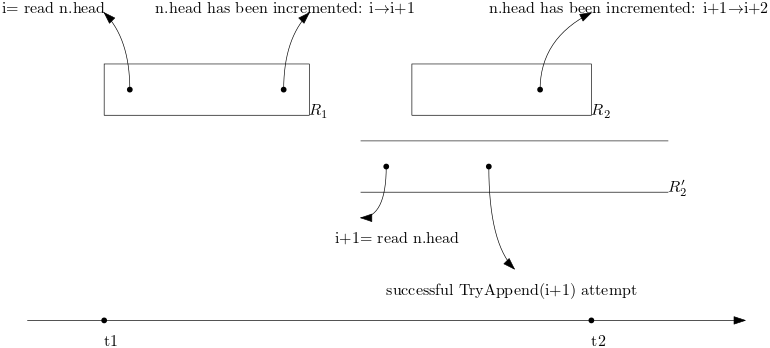
\includegraphics[width=6in]{pics/compactdouble.png}
  \caption{$t1<$ $r_1$ reading head $<$ incrementing \nf{n.head} from $i$ to $i+1$ $<$ $R_2^\prime$ reading head $<$ \nf{TryAppend(i+1)} $<$ incrementing \nf{n.head} from $i+1$ to $i+2$ $<t2$}
\end{figure}
\it{this chain with more depth should be in the proof}

%  Block \nf{new} is created of new established subblocks of children of \nf{n}(Lemma \ref{lem::createBlock}, Line 46). If \nf{CAS} in Line 48 succeeds then by Lemma~\ref{lem::trueRefresh} new established blocks will be in \nf{n}.
  
\begin{corollary}[Propagate Step] \label{doublyRefresh}
All operations in \nf{n}'s children's established blocks before line \ref{firstRefresh} are guaranteed to be in \nf{n}'s established blocks after line~\ref{secondRefresh}.
\end{corollary}
\begin{proof}
Lines \ref{firstRefresh} and \ref{secondRefresh} satisfy the preconditions of Lemma \ref{doubleRefresh}.
\end{proof}

\begin{corollary}
  After \nf{Append(blk)} finishes \nf{ops(blk)}$\subseteq$\nf{ops(root.blocks[x])} for some \nf{x} and only one \nf{x}.
\end{corollary}
\begin{proof}
  Follows from Lemma \ref{doubleRefresh}, \ref{append}.
\end{proof}

\begin{lemma}[Block Size Upper Bound]\label{blockSize}
Each block contains at most one operation from each processs.
\end{lemma}
\begin{proof}
By proof of contradiction, assume there are more than one operation from process $p$ in block $b$ in node $n$. A process cannot invoke more than one operations concurrently. From $p$ 's operations in $b$, let $op_1$ be the first operation invoked and $op_2$ be the second one. Note that it is terminated before $op_2$ started. So before appending $op_2$ to the tree $op_1$ exists in every node from the path of $p$'s leaf to the root. So there is some block $b^\prime$  before $b$ in $n$ containing $op_1$. $op_1$ existing in $b$ an $b^\prime$ contradicts with \ref{append}.
\end{proof}

\begin{lemma}[Subblocks Upperbound]\label{subBlocksBound}
Each block has at most $p$ direct subblocks.
\end{lemma}
\begin{proof}
  It follows directly from Lemma \ref{blockSize} and the observation that each block contains at least one operation, induced from Line~\ref{addOP}. 
\end{proof}


\begin{definition} [Ordering of operations inside the nodes] \label{ordering}
$\blacktriangleright$ Note that processes are numbered from 1 to $p$, left to right in the leaves of the tree and from Lemma \ref{blockSize} we know there is at most one operation from each process in a given block.

\begin{itemize}
\item We call operations strictly before $op$ in the sequence of operations $S$, prefix of the $op$.
  \item $E(n,b)$ is the sequence of enqueue operations $\in$ \nf{ops(n.blocks[b])} ordered by their process id.
  \item $E(n,b,i)$ is the $i$th enqueue in $E(n,b)$.
  \item $D(n,b)$ is the sequence of dequeue operations $\in$ \nf{ops(n.blocks[b])} ordered by their process id.
  \item $D(n,b,i)$ is the $i$th enqueue in $D(n,b)$.
\item Order of the enqueue operations in $n$: $E(n)=E(n,1).E(n,2).E(n,3)...$
\item $E(n,i)$ is the $i$th enqueue in $E(n)$.
\item Order of the dequeue operations in $n$: $D(n)=D(n,1).D(n,2).D(n,3)...$
\item $D(n,i)$ is the $i$th dequeue in $D(n)$.
\item Linearization: $L=E(root,1).D(root,1).E(root,2).D(root,2).E(root,3).D(root,3)...$
\end{itemize}
\end{definition}
\it{Note that in the non-root nodes we only order enqueues and dequeues among the operations of their own type. Since \nf{GetENQ()} only searches among enqueues and \nf{IndexDEQ()} works on dequeues.}

\begin{lemma}[Get correctness] \label{get}
If \nf{n.blocks[b].num\sub{enq}$\geq$i} then \nf{n.GetENQ(b,i)} returns $E(n,b,i)$.
\end{lemma}
\begin{proof}
We are going to prove this lemma by induction on the height of the tree. The base case for the leaves of the tree is pretty straight forward. Since leaf blocks contain exactly one operation then only \nf{GetENQ(b,1)} can be called on leaves. \nf{leaf.GetENQ(b,1)} returns the operation stored in the $b$th block of leaf $l$. For non leaf nodes in Line 404 it is decided that the \nf{i}th enqueue in block \nf{b} of internal node \nf{n}resides in the left child or the right child of \nf{n}. By definition of $E(n,b)$ operations from the left child come  before the operations of the right child. Having \nf{sum\sub{enq}}, the prefix sum of the number of enqueues we can compute the direct subblock containing the enqueue we are finding for with binary search. Then \nf{n.child.GetENQ( block containing, order in the block)} is invoked which returns the correct operation by the hypothesis of the induction.
\end{proof}
\textit{I'm not sure it is going to be long and boring to talk about the parameters, since the reader can find out them.}

\begin{lemma}[DSearch correctness] \label{dsearch}
If \nf{root.blocks[end].num\sub{enq}}$\geq$\nf{i} and $E(root, i)$ is the response to some \nf{Dequeue()} in \nf{root.blocks[end]} then \nf{DSearch(i, end)} returns \nf{b} such that \nf{root.blocks[b]} contains $E(root,b,i)$ in $\Theta(\log$(\nf{root.blocks[b].\size+root.blocks[end].\size}) steps.
\end{lemma}
\begin{proof}
First we show \nf{end-b}$\leq$\nf{root.blocks[b].\size+root.blocks[end].\size}. We know each block size is greater than 0. So every block in \nf{root.blocks[b..end]} contains at least one \nf{Enqueue()} or one \nf{Dequeue()}. There cannot be more than \nf{root.blocks[b].\size} \nf{Dequeue()}s in \nf{root.blocks[b+1..end-1]}, since the queue would become empty after bth block end before end and $E(n,i)$ could not be the response to to some \nf{DEQ} in \nf{end}. And since the lentgh of the queue would become \nf{root.blocks[end].\size} in the end so there cannot be more than \nf{root.blocks[end].\size} Dequeus in \nf{root.blocks[b..end]}. Cause if there was more then the end's lenght would become more than \nf{root.blocks[end].\size}.

Now that we know there are at most \nf{root.blocks[b].\size+root.blocks[end].\size} distance between end and b then with doubling search  in log\nf{root.blocks[b].\size+root.blocks[end].\size} steps we reach a block \nf{c} that the \nf{c.sum\sub{enq}} is less than i and the distance between c and end is not more than $2\times$\nf{root.blocks[b].\size+root.blocks[end].\size}. So the binary search takes $\Theta(\log$\nf{root.blocks[b].\size+root.blocks[end].\size)}$)$ steps.
\end{proof}


%\begin{definition}
%An enqueue operation is \textit{finished} if its argument is returned by some process. A dequeue operation is \texttt{finished} if it returns \nf{null} or some value. Block \nf{b} is \textit{done} if all operations in \nf{ops(b)} are finished.
%\end{definition}
%\textit{Problem: we increment the \nf{num\sub{finished}} before returning and after the computing response. How to articulate the sentence above in a not confusing correct way?}
%
%\begin{lemma}[help]\label{help}
%After that \nf{TryAppend()} who is helping finishes, prefix for the blocks of \nf{root.blocks[root.FindMostRecentDone]} are done.
%\end{lemma}

\begin{lemma}[Computing SuperBlock]\label{superBlock}
After computing line \ref{computeSuper} of \nf{n.IndexDEQ(b,i)}, \nf{n.parent.blocks[superblock]} contains $D(n,b,i)$.
\end{lemma}
\begin{proof}
\begin{enumerate}
 \item Value read for \nf{super[b.group]} in line 418 is not null.\\$\blacktriangleright$
  Values \nf{c\textsubscript{dir}} read in lines 23, \nf{super} are set before incrementing in lines 26,27.

 \item \nf{super[]} preserves order from child to parent; if in a child block \nf{b} is before \nf{c} then \nf{b.group} $\leq$ \nf{c.group} and \nf{super[b.group]} $\leq$ \nf{super[c.group]}\\$\blacktriangleright$
  Follows from the order of lines 60, 48, 49.

% \item In a propagate step at most 2 different time values are read \\ If there are more than 2 numbers then the smallest number should have been propagated far before.
% \item There are at most $p^2$ blocks with same time value in a node. \\ At most p processes could die before line 27 and each contains at most p elements.
 \item \nf{super[i+1]-super[i]}$\leq p$
\\$\blacktriangleright$
 In a Refresh with successful CAS in line 46, \nf{super} and \nf{counter} are set for each child in lines 48,49. Assume the current value of the counter in node \nf{n} is \nf{i+1} and still \nf{super[i+1]} is not set. If an instance of successful \nf{Refresh(n)} finishes \nf{super[i+1]} is set a new value and a block is added after \nf{n.parent[sup[i]]}. There could be at most $p$ successful unfinished concurrent instances of \nf{Refresh()} that have not reached line 49. So the distance between \nf{super[i+1]} and \nf{super[i]} is less than $p$.

 \item Superblock of \nf{b} is within range $\pm 2p$ of the \nf{super[b.time]}.
\\$\blacktriangleright$
\nf{super[i]} is the index of the superblock of a block containing block b, followed by Lemma \ref{superCounter}. It is trivial to see that \nf{n.super} and \nf{n.b.counter} are increasing. \nf{super(b)} is the real superblock of b. \nf{super(t]} is the index of the superblock of the last block with time \nf{t}. If \nf{b.time} is \nf{t} we have:
$$super[t]-p\leq super[t-1]\leq super(t-1] \leq super(b) \leq super(t+1)\leq super(t+1]\leq super[t]+p$$

\end{enumerate}
\end{proof}
We call the dequeues that return some value \it{non-null dequeues}. $r$th non-null dequeue returns the element of th $r$th enqueue. We can compute \# non-null dequeues in the prefix for a block this way: \#non-null dequeues= \size - \#enqueues. Note that the $i$th dequeue in the given block is not a non-null dequeue.

\begin{lemma}[Index correctness]
 \nf{n.IndexDEQ(b,i)} returns the rank in $D(root)$ of $D(n,b,i)$.
\end{lemma}
\begin{proof}
We can see the base case \nf{root.IndexDEQ(b,i)} is trivial.
  \nf{n.IndexDEQ(b,i)} computes the superblock of the $i$th Dequeue in the $b$th block of \nf{n} in \nf{n.parent}(Lemma \ref{superBlock}). Then the order in $D(n.parent, superblock)$ is computed and \nf{index()} is called on \nf{n.parent} recursively. It is easy to see why the second is correct. Correctness of computing superblock comes from Lemma \ref{superBlock}.\size
\end{proof}
\textit{Do I need to talk about the computation of the order in the parent which is based on the definition of ordering of dequeues in a block?}

\begin{lemma}[Search Ranges]\label{search}
  Preconditions of all invocation of \nf{BSearch} are satisfied.
\end{lemma}
\begin{proof}
  
Line 83: \nf{Get(i)} is called if the result of a dequeue is not null. The search is among all blocks in the root.

Line 88: This search tries to find the ith enqueue, knowing that it is in the left child. Search is done over the left subblocks. The start and end of the range are followed by definition. Line 92 is the same.

Line 101: Here, the goal is to find the superblock. We know the distance between answer and the \nf{super[i]} is at most $p$, since at most $p$ processes could die.

\end{proof}

\begin{lemma}[Computing Queue's Head block] \label{computeHead}
  Let $S$ be the state of an empty queue if the operations in prefix in $L$ of $i$th dequeue in $D(root,b)$ are applied on it. \nf{FindResponse()} returns \nf{(b, i)} which $E(root, b, i)$ is the the head of the queue in $S$. If the queue is empty in $S$ then it returns \nf{<-1,-->}.
  \end{lemma}
\begin{proof}
  The \size of the queue if the operations in the prefix for the $b$th block in the root are applied with the order of $L$ is stored in the \nf{root.blocks[b].\size}. It is computed while creating the block in Line~\ref{computeLength}. If the \size of a queue is greater than 0 then a \nf{Dequeue()} would decrease the \size of the queue, otherwise the \size of the queue remains 0. Having \size of the queue after the previous block and number of enqueues and dequeues in the block, Line~\ref{computeLength} computes wether the queue becomes empty or the \size of it.
\end{proof}
\framebox[1.1\width]{HOW?} How to prove mathematicaly that \nf{ax(root.blocks[i-1].\size + b.num\sub{enq} - b.num\sub{deq}, 0)} is the \size of the queue after the block. I can only explain it here.
%\begin{proof}
%  \nf{head} is incremented in lines 51, 54 after trying to append a block to the index of the last \nf{head} read. If it was successful, we have to do this, but if it was unsuccessful, it means it has appended to the index before, so we have to update the \nf{head}. If a process dies before line 51, another process will increment \nf{head} in line 54.
%\end{proof} 

\begin{lemma}[Validity of \nf{super} and \nf{counter}]\label{superCounter}
If \nf{super[i] $\neq$ null}, then \nf{super[i]} in node \nf{n} is the index of the superblock of a block with \nf{time=i}$\pm$\nf{p}.
\end{lemma}
%\begin{proof}
%After a successful CAS in line 46 \nf{super} and \nf{counter} are modified in both children. \nf{super[i]} is supposed to be the superblock of a block with \nf{time}=i and \nf{counter} is the timer in each node. \nf{super[i]} and \nf{counter=i} are expected to update after a bunch of blocks with \nf{time=i} have been aggregated together into a block in the parent. If the process dies before line 48 these values remain unchanged and incoming blocks will get the same \nf{time}. We claim that our algorithm still works since at most $p$ processes die and it will not change our complexity. If a process dies right after line 48, then \nf{counter} will remain the same and \nf{super[i]} is correct. Furthermore we are sure that when \nf{super[i]} is read it will not be \nf{null}.
%\end{proof}



\begin{lemma}[Root search range]\label{rootRange}
  \nf{root.size-root.FindMostRecentDone()} is $O(p^2+q)$, which $p$ is \# processes and $q$ is the \size of the queue.
\end{lemma}

\begin{theorem}[Main]
The queue implementation is linearizable.
\end{theorem}
%\begin{proof}
%  We show that the ordering $L$ stored in the root, satisfies the properties of a linearizable ordering.
%  \begin{enumerate}
%    \item If $op_1$ ends before $op_2$ begins in $E$, then $op_1$ comes before $op_2$ in $T$.\\$\blacktriangleright$ This is followed by Lemma \ref{append}. The time $op_1$ ends it is in root, before $op_2$, by Definition \ref{ordering} $op_1$ is before $op_2$.
%    \item Responses to operations in $E$ are same as they would be if done sequentially in order of $L$. \\$\blacktriangleright$ Enqueue operations do not have any response so it does no matter how they are ordered. It remains to prove  Dequeue $d$ returns the correct response according to the linearization order. By Lemma \ref{computeHead} it is deduced that the head of the queue at time of the linearization of $d$ is computed properly. If the Queue is not empty by Lemma \ref{get} we know that the returning response is the computed index element.
%  \end{enumerate} 
%\end{proof}

\begin{lemma}[Time analysis]
  \nf{n.GetEnq(b,i), n.Index(b,i)} take $O(\log^2 p)$ steps. Search in the root may take $O(\log Q+ p^2)$ steps. Helping is done every $p^2$ block appended to the root and takes $p\times \log^2p$ steps. Amortized time consumed for helping by each process is $O(\log^2 p)$.
\end{lemma}

\end{document}






